
\section{\hspace*{3pt}  Topology Description of the Wikipedia Category Graph}

A graph-theoretic analysis of the \gls{wcg} was carried out to describe the topology of the graph and to estimate whether graph-based techniques for semantic analysis and information retrieval can be applied to the Wikipedia Category Graph.

The inspiration for this section comes from the work of Zesch and Gurevych\cite{zesch2007analysis}, where they showed that the \gls{wcg} is a scale-free, small-world graph, like other semantic networks such as WordNet or Roget’s thesaurus. They concluded that the \gls{wcg} can be used for \gls{nlp} tasks, where other semantic networks have been traditionally employed\cite{zesch2007analysis}.

Although their work has been useful in supporting many types of research in the recent years, the analysis was performed in a German Wikipedia version of 2007. The idea behind our updated review is to understand if the latest version of Wikipedia in English also presents the same characteristics. We also expect to obtain insights on how the structure of the \gls{wcg} can influence the proposed method and guide the development of future work.



\subsection{\hspace*{3pt} Graph Density}

The Wikipedia Category Graph assembled for the experiments contains $1,475,806$ vertices and $4,091,417$ edges. Each vertex represents a category and each edge represents a relationship of the type ``Subcategory Of". 


The density $D$ of $G$ is the ratio of edges in $G$ to the maximum possible number of edges, defined in a directed graph as  
\begin{equation}
D={\frac  {|E|}{|V|\,(|V|-1)}}
\end{equation} where $V$ is the set of nodes and $E$ is the set of edges.

A graph is said to be dense when the number of existing edges is close to the number of possible edges. In the Wikipedia Category Graph the density is $1.878519 * 10^{-6}$.


\subsection{\hspace*{3pt} Degree Analysis}


If we observe a node in a directed graph, it is possible to see edges converging in the node and edges diverging from the node. An incoming edge and an outgoing edge can mean very different things, but in the Wikipedia Category Graph they both denote the direction of the relationship ``is subcategory of". 

The indegree of node $v$ is the total number of connections onto node $v$.
On the other side, the outdegree of node $v$ is the total number of connections coming out from node.

In both cases, the sum is the result of all other nodes $j$ in the graph. It is also possible to sum indegrees and outdegrees to get the total number of connections of a node, which constitutes its total degree.

The average indegree, outdegree and total degree for each vertex in the Wikipedia dataset are $2.78\pm0.142$, $2.78\pm0.001$ and $5.573\pm0.001$ respectively. 

\subsubsection{\hspace*{3pt}  Degree Distribution}

Large graphs such as the \gls{wcg} can be very complex structures, as the connections among the nodes can present complicated patterns. 
While studying complex networks, it is common to develop simplified measures that capture some elements of the structure. In this context, the degree distribution of complex network is often described. 

The degree distribution of a graph is the probability distribution that a randomly chosen node will have a degree $k$. 

In directed graphs the degree distribution is a two-dimensional distribution, so that $P_{\text{deg}}(k^{\text{in}},k^{\text{out}} ) =$ the portion of nodes in the graph with indegree $k^{\text{in}}$ and outdegree $k^{\text{out}}$

Figure \ref{fig:in-and-out-degree} shows the degree distribution for the Wikipedia Category Graph in log-log\footnote{
A two-dimensional graph of numerical data that uses logarithmic scales on both the horizontal and vertical axes. 
} plot. The $x$-axis shows the degree while the $y$-axis shows the count of nodes with such degree. 

\begin{figure}[!h]
\centering
\begin{subfigure}{0.49\textwidth}
\centering
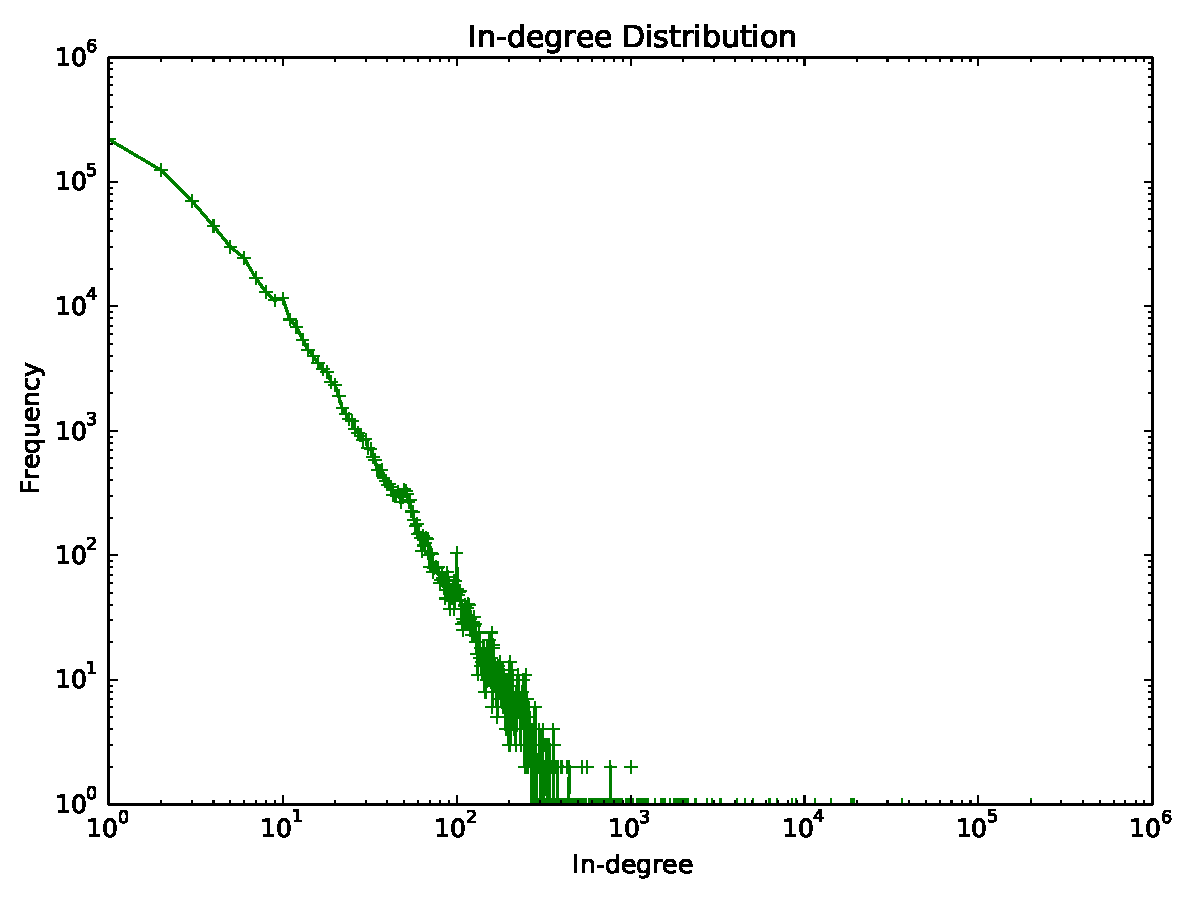
\includegraphics[width = \textwidth]{wikipedia-in-deg-dist.pdf}
\caption{Distribution of indegree}
\label{fig:left}
\end{subfigure}
\begin{subfigure}{0.49\textwidth}
\centering
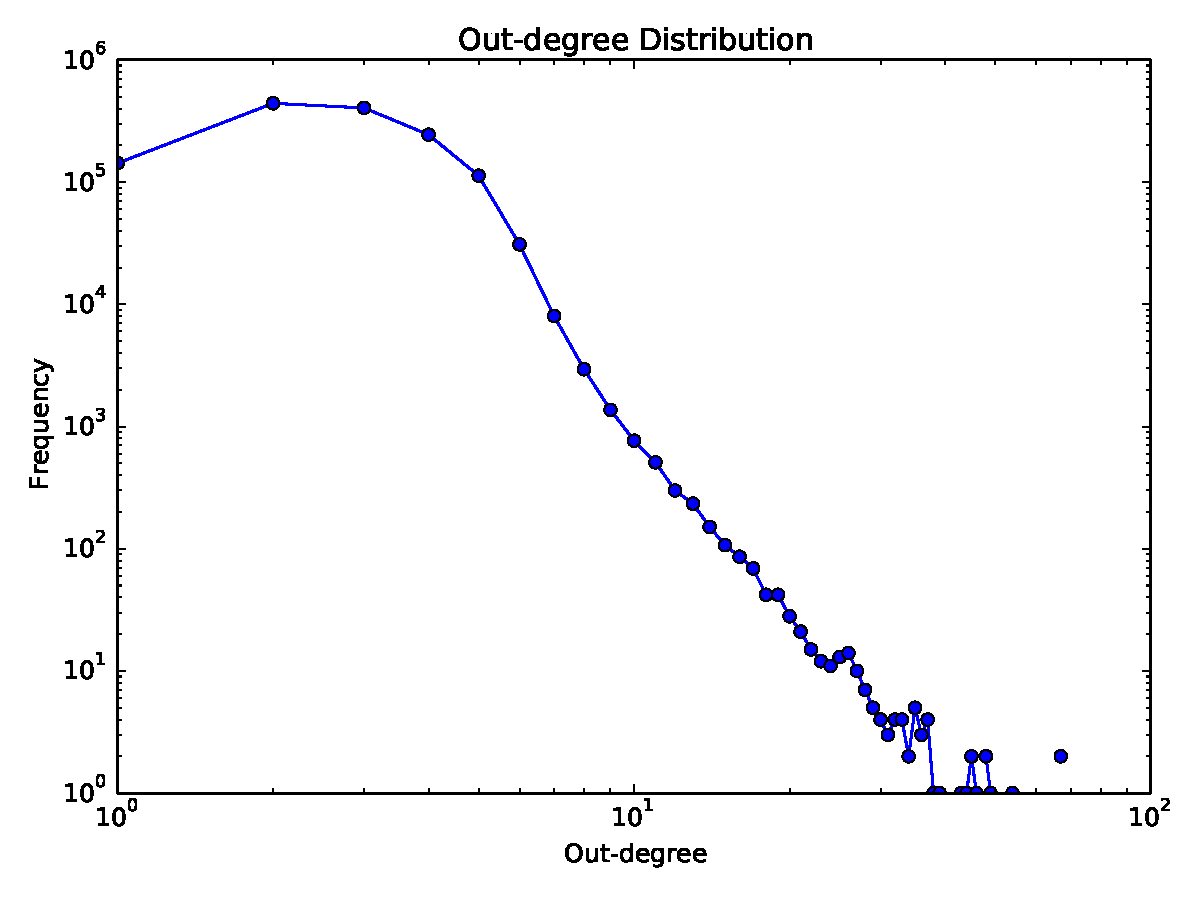
\includegraphics[width = \textwidth]{wikipedia-out-deg-dist.pdf}
\caption{Distribution of outdegree}
\label{fig:right}
\end{subfigure}
\caption{Indegree and outdegree distributions}
\label{fig:in-and-out-degree}
\end{figure}
Natural occurring networks tend to show a power-law distribution\footnote{A relationship between two variables such that one is proportional to a fixed power of the other.} which means that the fraction $P(k)$ of nodes in the graph having $k$ connections to other nodes varies as a power of some attribute $\alpha$, as in: 
\begin{equation}
P(k)=Ck^{-\alpha}
\end{equation}

This form of $P(k)$ decreases slowly as the degree $k$ increases, which multiplies the likelihood of finding nodes with a considerable degree.

Due to the fact that power-law networks do not have a typical degree, they are referred to as scale invariants or scale-free networks, which are characterized by the presence of large hubs\cite{mihalcea2011graph}. 

A method for determining the coefficient of the power law is defined in \cite{clauset2009power} as \begin{equation}
\alpha = 1 +n\left[\sum_{i=1}^n\ln\frac{x_i}{x_{\min}}\right]^{-1}
\end{equation}
where $x_{\min}$ is a lower cutoff, below which the power law cannot be observed. 


\begin{table}[ht!]
\centering
\begin{tabular}{@{}lll@{}}
\toprule
           & $\alpha$ & $x\_{min}$ \\ \midrule
in-degree  & 2,4124 & 10         \\
out-degree & 4,5603 & 12         \\ \bottomrule
\end{tabular}
\caption{Power-law parameters of the Wikipedia Category Graph}
\label{tab:power-law-params}
\end{table}

Based on the analysis of the \gls{wcg} degree distribution, as presented by the plot in figure \ref{fig:in-and-out-degree} and the exponent displayed in table \ref{tab:power-law-params}, it is demonstrated that the Wikipedia Category Graph nodes follow fit in a power-law distribution, hence we can consider it as a scale-free network.  

\subsubsection{\hspace*{3pt} Assortativity}

Regarding the degree distribution in a graph $G$, we can also determine the assortativity coefficient $r$, which measures how vertices of different types are preferentially connected amongst themselves. The assortativity coefficient \cite{newman2003mixing} is the Pearson correlation coefficient of degree between pairs of linked nodes. Positive values of $r$ indicate a correlation between nodes of similar degree, while negative values indicate relationships between nodes of different degree. In general, $r$ lies between -1 and 1. When $r = 1$, the network is said to have perfect assortative mixing patterns, when $r = 0$ the network is non\-assortative, and when  $r=-1$ the network is completely disassortative.

The assortativity coefficient for our graph for indegree, outdegree and total degree are  respectively: 
$-0.0034$, $0.0898$, $0.0051$. 

Assortativity is high when high-degree nodes tend to connect to other high-degree nodes, and it is low (i.e., negative) when high-degree nodes are linked to low-degree nodes. An assortativity of 0 indicates no correlation between the degrees of the nodes.

In this case, since the assortativity regarding indegree and outdegree is very low, we can infer that there is no preferential attachment in the \gls{wcg}, meaning that nodes with a high degree will not necessarily be connected to other nodes with high degree.  Hence, the hubs are distributed along the structures and not concentrated in a same region of the graph.


\subsection{\hspace*{3pt} Path lengths}

A path in a graph is a sequence of alternating nodes and edges that starts with a node and ends with another node in such a way that adjacent nodes and edges in the sequence are incidental to each other \cite{newman2010networks}. Nodes or edges can appear in the same path multiple times, and the number of edges in a path is the length of that given path. If a graph is connected, then any node can be reached via a finite-length path starting from any other node. The shortest path between a pair of nodes is called a geodesic path and there can be more than one such path.

The average path length, a concept in the field of network topology, is defined as the average number of steps in the shortest paths for all possible pairs of nodes in the graph. In directed graphs, the average path length is calculated as follows:

\begin{equation}
l_{G}={\frac  {1}{2 * n\cdot (n-1)}}\cdot \sum _{{i\neq j}}d(v_{i},v_{j})
\end{equation}

where $d(v_{1},v_{2})$ denotes the shortest distance between $v_1$ and $v_2$ and $n$ is the number of vertices in the graph $G$. 

If two nodes are disconnected (i.e., no path exists between them), the path length between these nodes is infinite. Consequently, if a graph contains disconnected components, the average shortest path length $l_G$ tends to infinity. 
Given that the \gls{wcg} is not completely connected, to avoid infinity, we calculated the average shortest path length for the largest connected component. As a result, the $l_G$ is $20,9343$. The shortest path length distribution is displayed in figure \ref{fig:path-distribution} where the y-axis represents the number of nodes and the x-axis represents the number average path length.



\begin{figure}[H]
  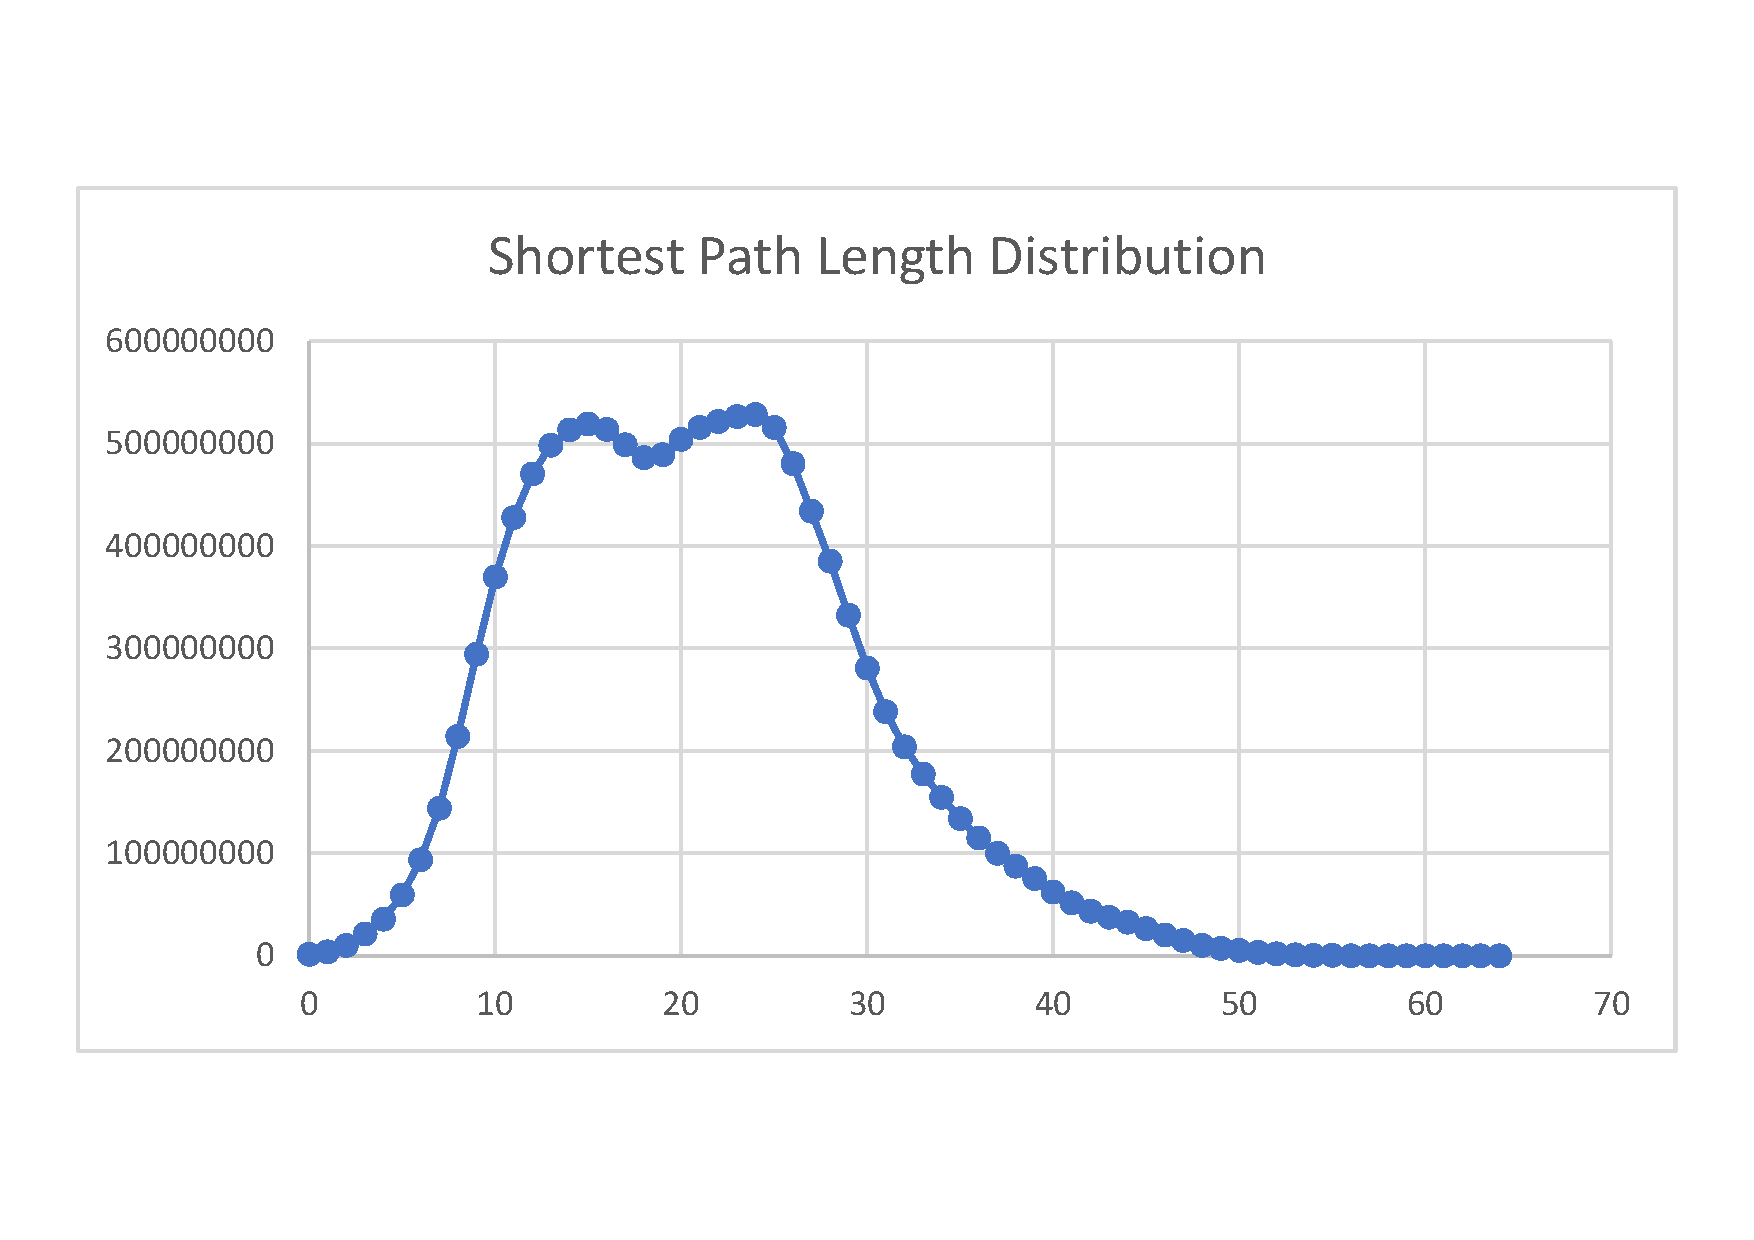
\includegraphics[width=\linewidth]{path_frequency2}
  \caption{Shortest path length distribution on th Wikipedia Category Graph}
  \label{fig:path-distribution}
\end{figure}


\subsubsection{\hspace*{3pt} Graph Diameter}

The diameter $d$ of a graph $G$ is the maximum topological distance that can be found between two nodes in $G$. In order to find the diameter of a graph, the shortest path between each pair of vertices needs to be determined first. The greatest length of any of these paths is the diameter of the graph. Alternatively, we can define it as 
\begin{equation}
d=\max _{v\in V}\epsilon (v)
\end{equation}
It is worth noticing that the distance is determined based on the graph direction. In the Wikipedia Category Graph, the maximum topological distance is $52$ and the nodes with the longest shortest path are Bengali Culture and Politics of Bangladesh. 


\subsection{\hspace*{3pt} Small World}

A small-world is a type of graph in which most nodes are not neighbors between them, but the neighbors of any given node are likely to be neighbors of each other, and most nodes can be reached from every other node by a small number of steps. Specifically, a small-world network is defined to be a network where the typical distance $L$ between two randomly chosen nodes grows proportionally to the logarithm of the number of nodes $N$ in the graph $G$ while the clustering coefficient is not small.

Formally, a graph $G$ with $n$ nodes and $m$ vertices is said to be a small-world if it has a similar path length but greater clustering of nodes than an equivalent Erdös-Rényi (E–R) random graph with the same $m$ and $n$. Let $L_g$ be the mean shortest path length of $G$ and $cc_{2_g}$ its clustering coefficient using the equation \ref{eq:cc2}. Let $L_{rand}$ and  $cc_{2_{rand}}$ be the corresponding quantities for the corresponding E–R random graph. According to the empirical experiments performed in \cite{watts1998collective}, a graph $G$ is said to be a small-world network if $L_g \ge L_{rand}$ and $ cc_{2_g} \gg cc_{2_{rand}}$.

In small-world graphs, the distance between any pair of nodes is relatively short while the level of transitivity, or clustering. is relatively high.



\subsubsection{\hspace*{3pt} Clustering Coefficient}

Another important metric for understanding the topology of a graph is its clustering coefficient. The clustering coefficient of a vertex represents the probability that if two of its neighbors are randomly chosen, they will also be connected by an edge. More precisely, if a vertex has $t$ neighbors, then there are $t(t-1)/2$ possible edges that connect those neighbors. The local clustering coefficient of a vertex is the fraction of the edges that actually appear in the graph (or 0 if the vertex has degree 0 or 1). Given the graph $G= (v,E)$ and a vertex $v \in V$, the clustering coefficient of $v$ is 

\begin{equation}\label{eq:cc1}
cc_1(v) = \dfrac{number of pairs of neighbors connected by edges}{number of pairs of neighbors}  
\end{equation} 

The clustering coefficient of a graph $G$ is the average of the local clustering coefficients $cc_1(v)$ of all vertices $v \in V$. The Wikipedia Category Graph has a clustering coefficient of $0.0461$. 

An alternative way of calculating the clustering coefficient of a graph is referred to as the global clustering coefficient or transitivity \cite{newman2001random}. Given the graph $G = (V,E)$ the global clustering coefficient of $G$ is
\begin{equation}\label{eq:cc2}
cc_2 = \dfrac{number of closed 2paths}{number of 2paths}
\end{equation} For the Wikipedia Category Graph, the global clustering coefficient is $0.0036\pm0.005$. 



\begin{table}[!h]
\centering
\begin{tabular}{@{}lllll@{}}
\toprule
    & $L_g$       & $L_{rand}$       & $cc_{2_g}$           & $cc_{2_{rand}}$        \\ \midrule
WCG & 20,9343 & 19,5389 & 0,003638604 & 2,03E-06 \\ \bottomrule
\end{tabular}
\caption{Empirical demonstration of small-worldness of WCG }
\label{small-worldness}
\end{table}

Therefore, the Wikipedia Category Graph exhibits a small-world behavior, with an average shortest path length close to that of a random network with the same size.